\lab{Newton's Method and Basins of Attraction}{Newton's Method}
\label{lab:NewtonsMethod}
\objective{Use Newton's Method to find zeros of a function.  Determine where an initial point will converge to based on basins of attraction.}

Newton's method finds the roots of functions; that is, it finds $\overline{x}$ such that $f\left(\overline{x}\right) = 0$.
This method can be used in optimization to determine where the maxima and minima occur. For example, it can be used to find the zeros of the first derivative.

\section*{Newton's Method}
Newton's method begins with an initial guess $x_0$. 
Successive approximations of the root are found with the following recursive sequence:
\[
x_{n+1} = x_n - \frac{f(x_n)}{f'(x_n)}.
\]
In other words, Newton's method approximates the root of a function by finding the x-intercept of the tangent line at $(x_n, f(x_n))$ (see Figure \ref{fig:newton}).

The sequence $\{x_n\}$ will converge to the zero $\overline{x}$ of $f$ if
\begin{enumerate}
\item $f$, $f'$, and $f''$ exist and are continuous,
\item $f'(\overline{x})\neq0$, and
\item $x_0$ is ``sufficiently close'' to $\overline{x}$.
\end{enumerate}
In applications, the first two conditions usually hold.
However, if $\overline{x}$ and $x_0$ are not ``sufficiently close,'' Newton's method may converge very slowly, or it may not converge at all.

\begin{figure}[h]
\label{fig:newton}
\centering
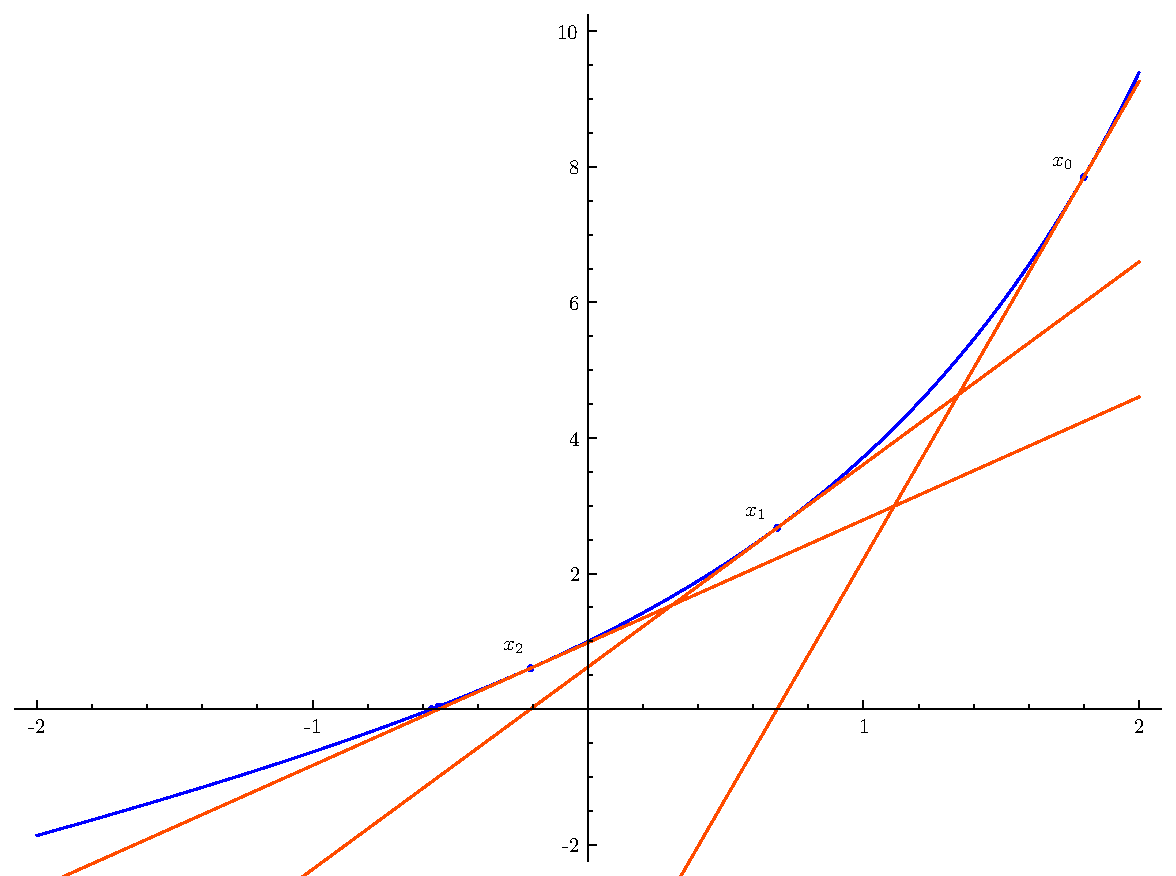
\includegraphics[width=\textwidth]{newton_iters}
\caption{An illustration of how two iterations of Newton's method work.}
\end{figure}

Newton's method is powerful because given the three conditions above, it converges quickly.
In these cases, the sequence $\{x_n\}$ converges to the actual root quadratically, meaning that the maximum error is squared at every iteration.

Let us do an example with $f(x) = x^2-1$. 
We define $f(x)$ and $f'(x)$ in Python as follows. 
\begin{lstlisting}
>>> import numpy as np
>>> from matplotlib import pyplot as plt
>>> f = lambda x : x**2 - 1
>>> Df = lambda x : 2*x
\end{lstlisting}
Now we set $x_0 = 1.5$ and iterate.
\begin{lstlisting}
>>> xold = 1.5
>>> xnew = xold - f(xold)/Df(xold)
>>> xnew
1.0833333333333333
\end{lstlisting}
We can repeat this as many times as we desire.
\begin{lstlisting}
>>> xold = xnew
>>> xnew = xold - f(xold)/Df(xold)
>>> xnew
1.0032051282051282
\end{lstlisting}
We have already computed the root 1 to two digits of accuracy.


\begin{problem}
\label{prob:newton_arr}
\leavevmode

Implement Newton's method with the a function called \li{Newtons_method()} that accepts the following parameters: a function $f$, an initial x-value, the derivative of the function $f$, the number of iterations of Newton's method to perform that defaults to 15, and a tolerance that defaults to $10^{-6}$.  
The function  returns when the difference between successive approximations is less than the tolerance or the max number of iterations has been reached.
\end{problem}

\begin{problem}
\begin{enumerate}
\label{prob:functions}

\item Newton's method can be used to find zeros of functions that are hard to solve for analytically.
Plot $f(x) = \frac{sin(x)}{x}-x$ on $[-4, 4]$. 
Note that this function can be made continuous on this domain by defining $f(0)=1$. 
Use your function \li{Newtons_method()} to compute the zero of this function to seven digits of accuracy.
\item Run \li{Newtons_method()} on $f(x)=x^{1/3}$ with $x_0=.01$. 
What happens and why?
Hint: The command \li{x**(1/3)} will not work when \li{x} is negative. 
Here is one way to define the function $f(x)=x^{1/3}$ in NumPy.
\begin{lstlisting}
f = lambda x: np.sign(x)*np.power(np.abs(x), 1./3)
\end{lstlisting}
\end{enumerate}
\end{problem}

\begin{problem}
Suppose that an amount of $P_1$ dollars is put into an account at the beginning of years $1, 2,..., N_1$ and that the account accumulates interest at a fractional rate $r$.  
(For example, $r = .05$ corresponds to $5\%$ interest.) 
Suppose also that, at the beginning of years $N_1 + 1, N_1 + 2, ..., N_1 + N_2$, an amount of $P_2$ dollars is withdrawn from the account and that the account balance is exactly zero after the withdrawal at year $N_1 + N_2$.
Then the variables satisfy the following equation:
\[
P_1[(1+r)^{N_1} - 1] = P_2[1-(1+r)^{-N_2}].
\]
If $N_1 =30, N_2 =20, P_1 =2000$, and $P_2 =8000$, use Newton's method to
determine $r$.
(From Atkinson Page 118)
\end{problem}

\begin{comment}
\begin{problem}
Extend your Newton's method even further so that it will work on systems of equations.
Suppose that $F: \mathbb{R}^n \rightarrow \mathbb{R}^n $.
The relevant equation is
\[
x_{i+1} = x_i - J^{-1}F(x_i)
\]
Note that you should not calculate the inverse Jacobian.
\li{scipy.linalg.solve(A,b)} gives you the solution $x$ to the equation $Ax=b$.
Use this fact to calculate $J^{-1}F$ from $J$ and $F$.
You should be able to make this function work whether or not the user inputs a Jacobian.
This also means that you will have to use your own \li{jacobian} function.
\end{problem}
\end{comment}

\section*{Backtracking}
There are times when Newton's method may not converge due to the fact that the step from $x_n$ to $x_{n+1}$ was too large and the zero was stepped over completely.  This was seen in Problem \ref{prob:functions} when using $x_0 = .01$ to find the zero of $f(x)=x^{1/3}$. In that example, Newton's method did not converge since it stepped over the zero of the function, produced $x_1 = -.02$ and each iteration got increasingly more negative.  To combat this problem of overstepping, backtracking is a useful tool.  Backtracking is simply taking a fraction of the full step from $x_n$ to $x_{n+1}$.  Define Newton's Method with the recursive sequence:
\[
x_{n+1} = x_n - \alpha\frac{f(x_n)}{f'(x_n)}
\]
and the vector version of Newton's Method as:
\[
x_{n+1} = x_n - \alpha{Df(x_n)}^{-1}{f(x_n)}.
\]
Previously, we have used $\alpha = 1$ in Newton's method.  Backtracking uses $\alpha < 1$ in the above sequences and allows us to take a fraction of the step when the step size is too big.
\begin{problem}
\begin{enumerate}

\item Modify your \li{Newtons_method()} function so that it accepts a parameter $\alpha$ that defaults to $1$ to allow backtracking.
\item Find an $\alpha < 1$ so that running \li{Newtons_method()} on $f(x)=x^{1/3}$ with $x_0=.01$ converges.  
(See Problem \ref{prob:functions}).
Return the results of \li{Newtons_method()}.


\end{enumerate}
\end{problem}

\begin{problem}
\begin{enumerate}

\item Create a \li{Newtons_vector()} function that performs Newton's method on vectors.
\item Bioremediation involves the use of bacteria to consume toxic wastes.
At steady state, the bacterial density $x$ and the nutrient concentration $y$ satisfy the system of nonlinear equations
\[
\gamma xy - x(1 + y) = 0,
\]
\[
 -xy + (\delta - y)(1 + y) = 0,
\]
where $\gamma$ and $\delta$ are parameters that depend on various physical features of the system. 
For this problem, assume the typical values $\gamma = 5$ and $\delta = 1$, for which the system has solutions at $(x, y) = (0, 1), (0, -1)$, and $(3.75, .25)$. 
Solve the system using Newton's method and Newton's method with backtracking. 
(Find an initial point where using $\alpha = 1$ converges to either $(0, 1)$ or $(0, -1)$ and using $\alpha < 1$ converges to $(3.75, .25)).$  
Use  matplotlib to demonstrate the tracks used to find the solution. (See Figure \ref{fig:contour_plot})
Hint: use starting values within the rectangle 
\[
{(x, y) : -.25 \leqslant x \leqslant .25, -.25 \leqslant y \leqslant .25}.
\]
(Adapted from problem 5.19 of M. T. Heath, Scientific Computing, an Introductory Survey, 2nd edition, McGraw?Hill, 2002 and the Notes of Homer Walker)
\end{enumerate}
\end{problem}

\begin{figure}[h]
\label{fig:contour_plot}
\centering
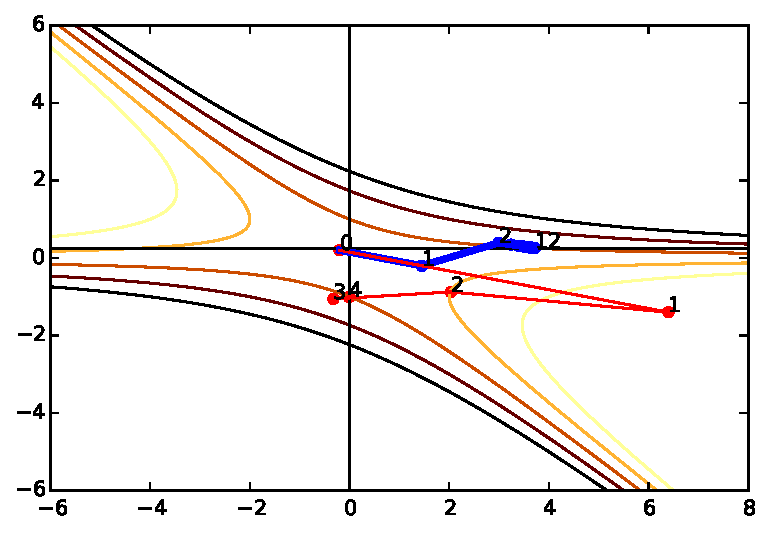
\includegraphics[width=\textwidth]{contour}
\caption{Starting at the same initial value results in convergence to two different solutions.  The red line converges to $(0,-1)$ with $\alpha = 1$ in $4$ iterations of Newton's method while the blue line converges to $(3.75,.25)$ with $\alpha < 1$ in $12$ iterations .}
\end{figure}

\section*{Basins of Attraction: Newton Fractals}
When $f(x)$ has many roots, the root that Newton's method converges to depends on the initial guess $x_0$.
For example, the function $f(x)=x^2-1$ has roots at $-1$ and $1$.
If $x_0<0$, then Newton's method converges to -1; if $x_0>0$ then it converges to 1 (see Figure \ref{fig:basins1}).
We call the regions $(-\infty, 0)$ and $(0, \infty)$ \emph{basins of attraction}.

\begin{figure}
\begin{center}
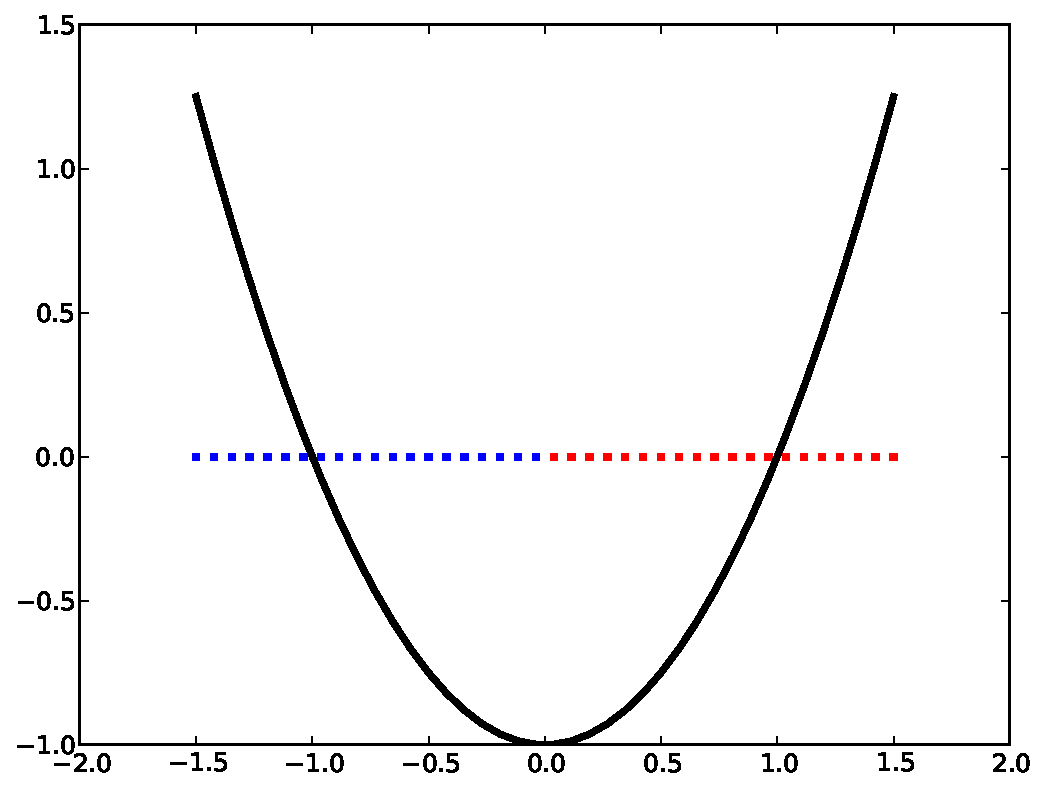
\includegraphics[scale=0.5]{basins1}
\caption{The plot of $f(x) = x^2 -1$ along with some values for $x_0$.
When Newton's method is initialized with a blue value for $x_0$ it converges to -1; when it is initialized with a red value it converges to 1.}
\label{fig:basins1}
\end{center}
\end{figure}

When $f$ is a polynomial of degree greater than 2, the basins of attraction are much more interesting.
For example, if $f(x) = x^3-x$, the basins are depicted in Figure \ref{fig:fractal_1d}.

\begin{figure}
\begin{center}
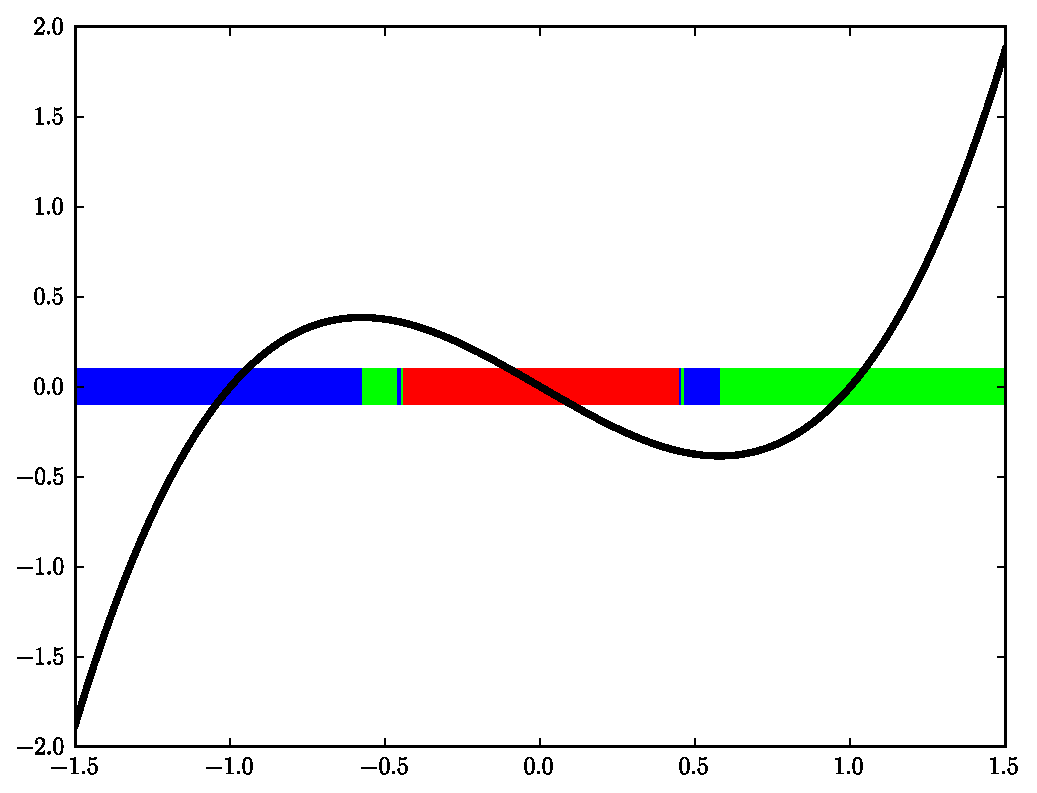
\includegraphics[scale=0.5]{fractal1d}
\caption{The plot of $f(x) = x^3 -x$ along with some values for $x_0$.
Blue values converge to $-1$, red converge to 0, and green converge to 1.}
\label{fig:fractal_1d}
\end{center}
\end{figure}

We can extend these examples to the complex plane. 
Newton's method works in arbitrary Banach spaces with slightly stronger hypotheses (see Chapter 7 of Volume 1), and in particular it holds over $\mathbb{C}$.

Let us plot the basins of attraction for $f(x) = x^3-x$ on the domain $\{a+bi \mid (a, b) \in [-1.5, 1.5] \times [-1.5, 1.5] \}$ in the complex plane.
We begin by creating a $700 \times 700$ grid of points in this domain. 
We create the real and imaginary parts of the points separately, and then use \li{np.meshgrid()} to turn them into a single grid of complex numbers.
\begin{lstlisting}
>>> xreal = np.linspace(-1.5, 1.5, 700)
>>> ximag = np.linspace(-1.5, 1.5, 700)
>>> Xreal, Ximag = np.meshgrid(xreal, ximag)
>>> Xold = Xreal+1j*Ximag
\end{lstlisting}
Recall that \li{1j} is the complex number $i$ in NumPy. 
The array \li{Xold} contains $700^2$ complex points evenly spaced in the domain.

We may now perform Newton's method on the points in \li{Xold}. 
\begin{lstlisting}
>>> f = lambda x : x**3-x
>>> Df = lambda x : 3*x**2 - 1
>>> Xnew = Xold - f(Xold)/Df(Xold)
\end{lstlisting}
After iterating the desired number of times, we have an array \li{Xnew} whose entries are various roots of $x^3-x$.

Finally, we plot the array \li{Xnew}. The result is similar to Figure \ref{fig:fractal_ex}.
\begin{lstlisting}
>>> plt.pcolormesh(Xreal, Ximag, Xnew)
\end{lstlisting}

Notice that in Figure \ref{fig:fractal_ex}, whenever red and blue try to come together, a patch of green appears in between.
This behavior repeats on an infinitely small scale, producing a fractal.
Because it arises from Newton's method, this fractal is called a \emph{Newton fractal}.

\begin{figure}
\begin{center}
\begin{subfigure}[b]{.49\textwidth}
\centering
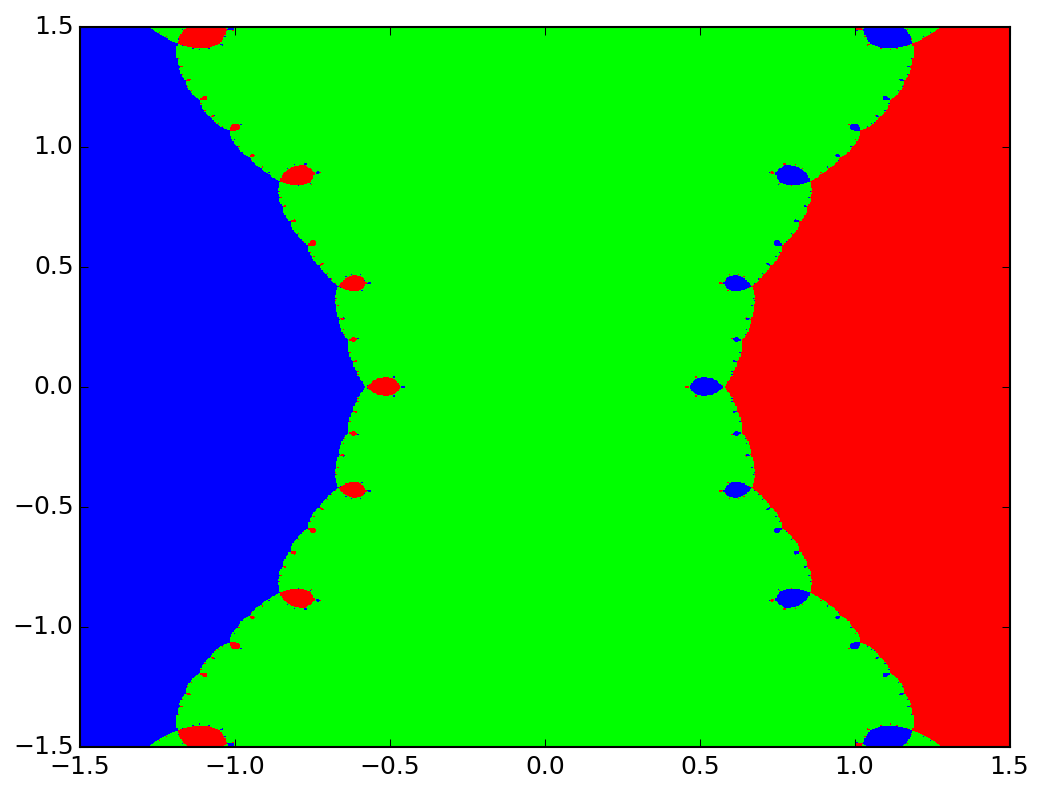
\includegraphics[width=\textwidth]{fractal_ex}
\end{subfigure}
\begin{subfigure}[b]{.49\textwidth}
\centering
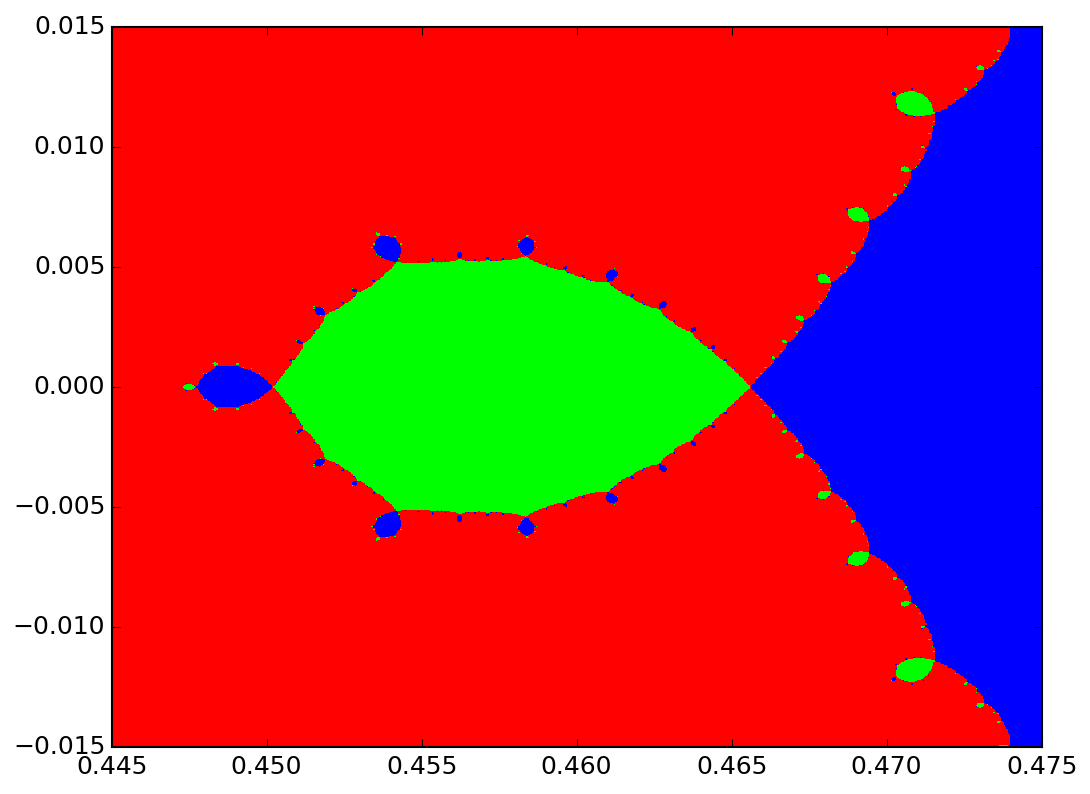
\includegraphics[width=\textwidth]{fractal_zoom}
\end{subfigure}
\caption{ Basins of attraction for $x^3-x$ in the complex plane. 
The picture on the right is a close-up of the figure on the left.}
\label{fig:fractal_ex}
\end{center}
\end{figure}

Newton fractals tell us that the long-term behavior of the Newton method is extremely sensitive to the initial guess $x_0$.
Changing $x_0$ by a small amount can change the output of Newton's method in a seemingly random way.
This is an example of \emph{chaos}.





\begin{problem}
\leavevmode

Complete the following function to plot the basins of attraction of a function.
\begin{lstlisting}
def plot_basins(f, Df, roots, xmin, xmax, ymin, ymax, numpoints=100, iters=15, colormap='brg'):
    '''Plot the basins of attraction of f.
    
    INPUTS:
    f       - A function handle. Should represent a function 
            from C to C.
    Df      - A function handle. Should be the derivative of f.
    roots   - An array of the zeros of f.
    xmin, xmax, ymin, ymax - Scalars that define the domain 
            for the plot.
    numpoints - A scalar that determines the resolution of 
            the plot. Defaults to 100.
    iters   - Number of times to iterate Newton's method. 
            Defaults to 15.
    colormap - A colormap to use in the plot. Defaults to 'brg'.    
    '''
\end{lstlisting}
You can test your function on the example $f(x) = x^3-x$ above. 

When the function \li{plt.pcolormesh()} is called on a complex array, it evaluates only on the real part of the complex numbers.
This means that if two roots of \li{f} have the same real part, their basins will be the same color if you plot directly using \li{plt.pcolormesh()}.

One way to fix this problem is to compute \li{Xnew} as usual.
Then iterate through the entries of \li{Xnew} and identify which root each entry is closest to using the input \li{roots}.
Finally, create a new array whose entries are integers corresponding to the indices of these roots.
Plot the array of integers to view the basins of attraction.  Hint: The roots of $f(x) = x^3-x$ are $[0,1,-1]$.
\end{problem}

\begin{problem}

Run \li{plot_basins()} on the function $f(x) = x^3-1$ on the domain $\{a+bi \mid (a, b) \in [-1.5, 1.5] \times [-1.5, 1.5] \}$. 
The resulting plot should look like Figure \ref{fig:fractal_hw}.  Hint: the roots of $f(x) = x^3-1$ are $[1,-1j^{1/3},1j^{2/3}]$.


\begin{figure}[H]
\begin{center}
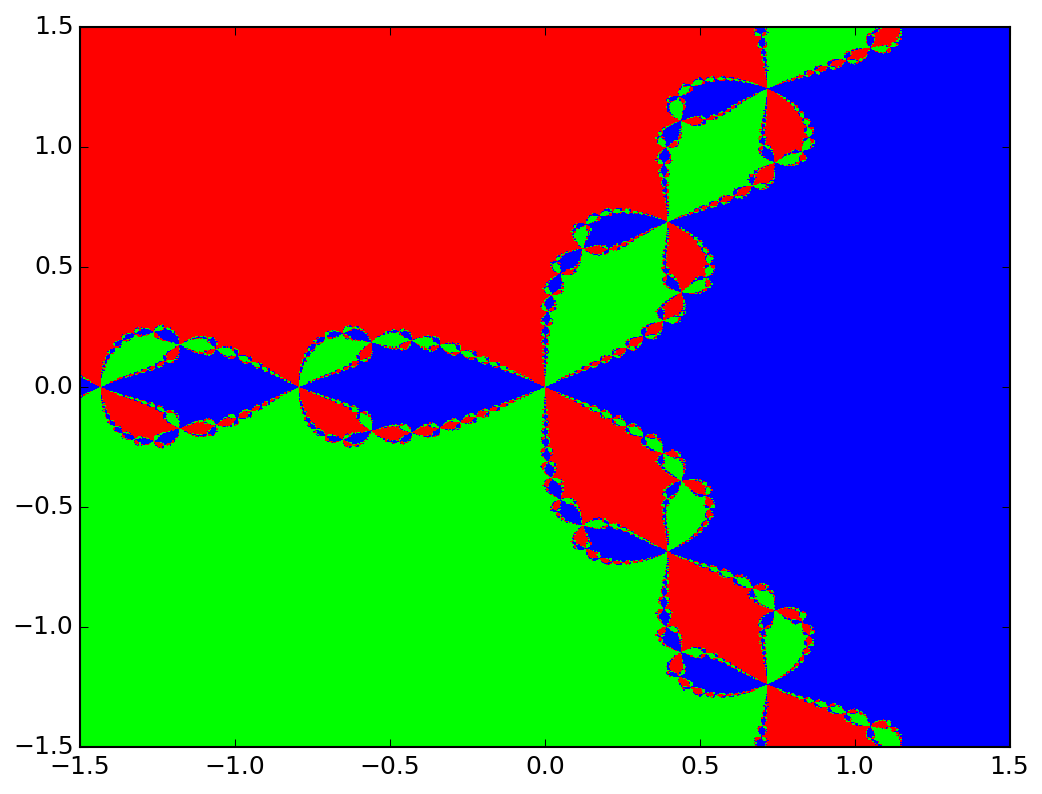
\includegraphics[scale=0.66]{fractal_hw}
\caption{Basins of attraction for $x^3-1$.}
\label{fig:fractal_hw}
\end{center}
\end{figure}
\end{problem}


% The remainder of the material has nothing to do with this lab, except that it mentions fractals.
\begin{comment}
Another well-studied fractal in the complex plane is the Mandelbrot set.
It is defined as the points $c \in \mathbb{C}$ for which the sequence
\[z_n = z_{n-1}^2 + c\]
is bounded.

\begin{problem}
Generate another grid of complex numbers on $[-1.5,.5]\times[-i,i]$.
Consider the recurrence relation $x_n = x_{n-1}^2 + c$.
Run this iteration 30 times with a resolution of $200 \times 200$ and display the plot.
\end{problem}
\end{comment}
